% dibuix_cilindre_1.tex
\documentclass{standalone}
\usepackage{tikz}
\usetikzlibrary{arrows.meta, decorations.markings}

\begin{document}

\begin{tikzpicture}[
    identified_edge/.style={
        decoration={
            markings,
            mark=at position 0.5 with {\arrow{Latex}}
        },
        postaction={decorate}
    },
    edge_label/.style={midway, auto, font=\small}
]

\def\squaresize{3}
\fill[gray!10] (0,0) -- (0.2 * \squaresize,\squaresize) -- (1.8 * \squaresize,\squaresize) -- (2 * \squaresize,0) -- cycle;
\node[anchor=center] at (\squaresize,0.5*\squaresize) {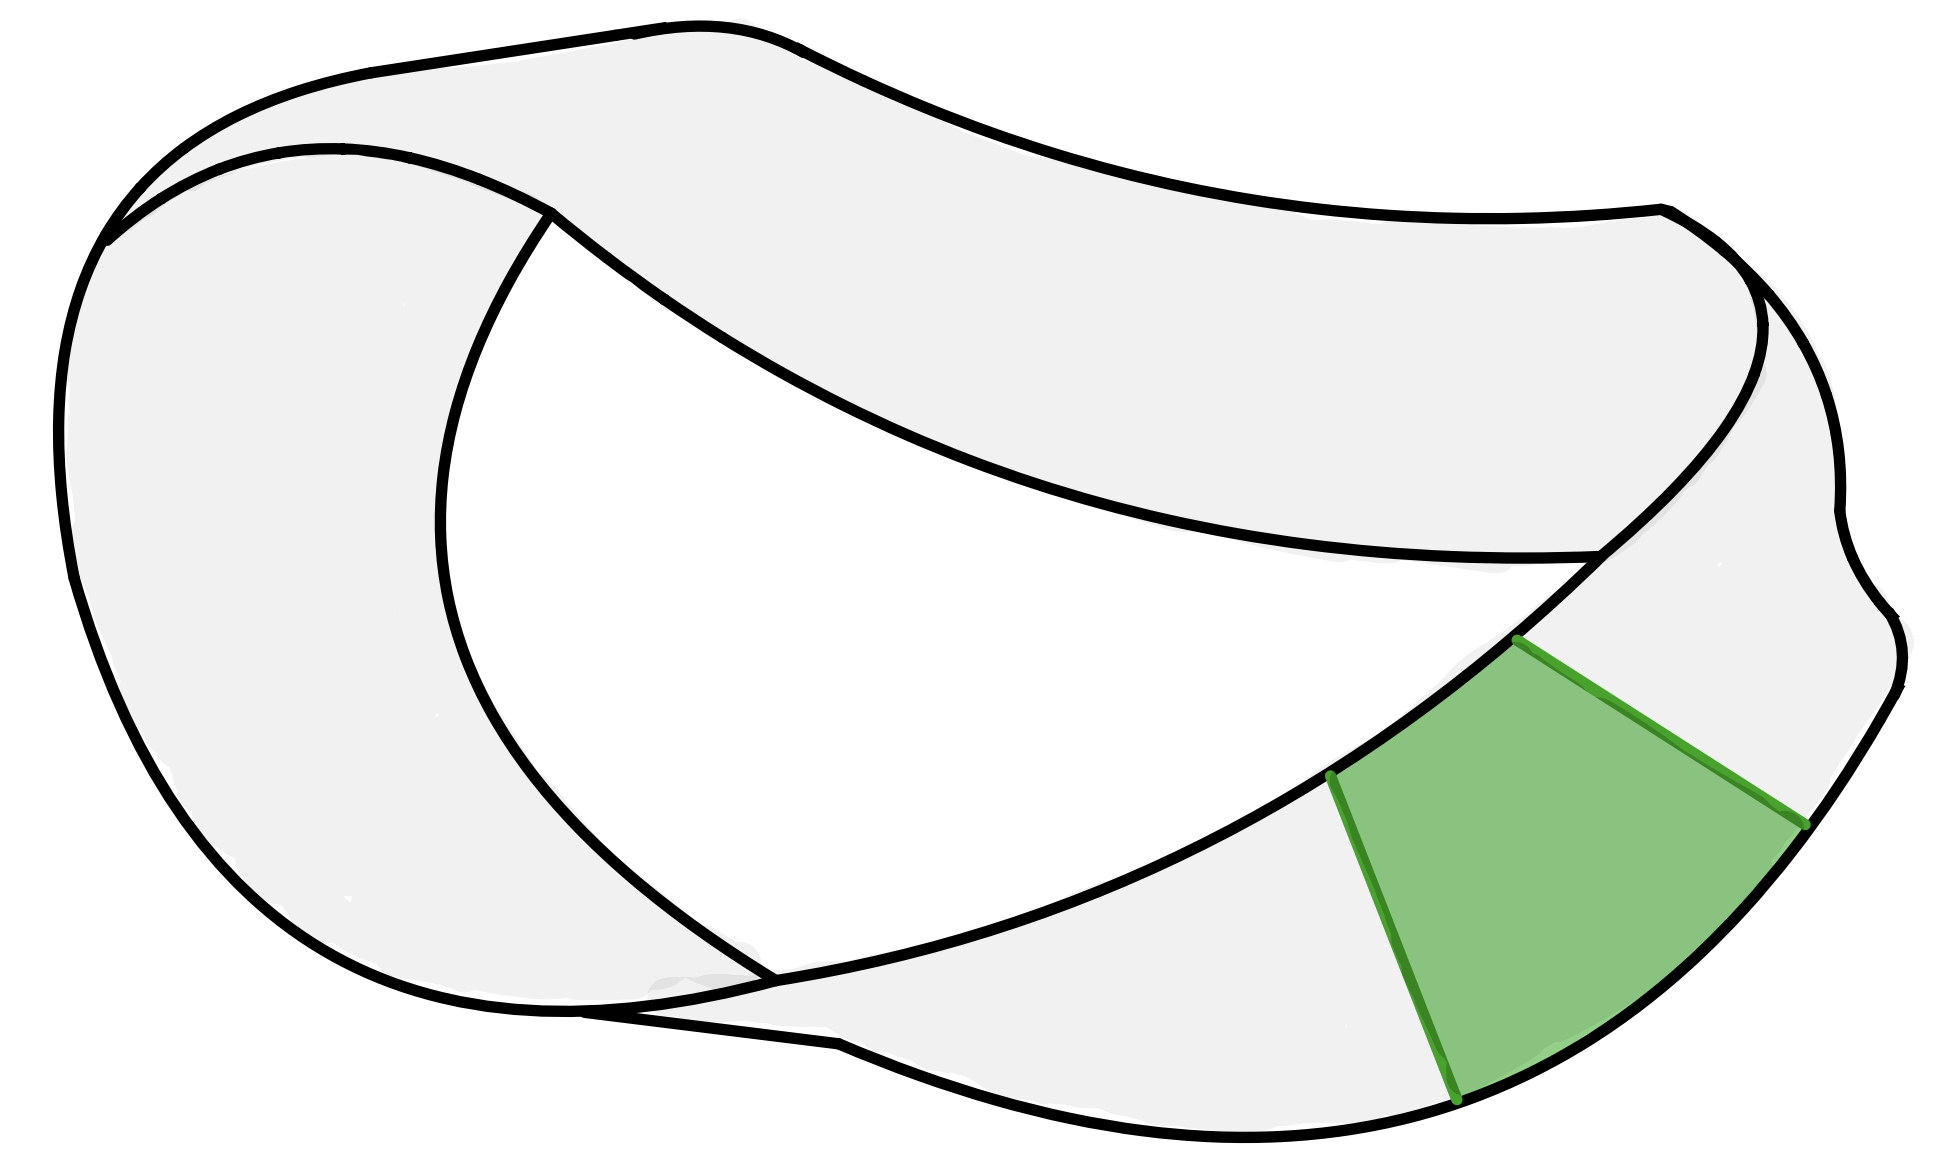
\includegraphics{verd.png}};
\node[green!50!black, scale=10] at (4.3*\squaresize, -0.9*\squaresize) {$\tau'$};
\node[scale=10] at (\squaresize, 0*\squaresize) {$\Omega$};


\end{tikzpicture}

\end{document}